\documentclass[14pt]{beamer}
\usepackage{./Estilos/BeamerUVM}
\usepackage{./Estilos/ColoresLatex}
\usetheme{Madrid}
\usecolortheme{default}
%\useoutertheme{default}
\setbeamercovered{invisible}
% or whatever (possibly just delete it)
\setbeamertemplate{section in toc}[sections numbered]
\setbeamertemplate{subsection in toc}[subsections numbered]
\setbeamertemplate{subsection in toc}{\leavevmode\leftskip=3.2em\rlap{\hskip-2em\inserttocsectionnumber.\inserttocsubsectionnumber}\inserttocsubsection\par}
% \setbeamercolor{section in toc}{fg=blue}
% \setbeamercolor{subsection in toc}{fg=blue}
% \setbeamercolor{frametitle}{fg=blue}
\setbeamertemplate{caption}[numbered]

\setbeamertemplate{footline}
\beamertemplatenavigationsymbolsempty
\setbeamertemplate{headline}{}


\makeatletter
% \setbeamercolor{section in foot}{bg=gray!30, fg=black!90!orange}
% \setbeamercolor{subsection in foot}{bg=blue!30}
% \setbeamercolor{date in foot}{bg=black}
\setbeamertemplate{footline}
{
  \leavevmode%
  \hbox{%
  \begin{beamercolorbox}[wd=.333333\paperwidth,ht=2.25ex,dp=1ex,center]{section in foot}%
    \usebeamerfont{section in foot} {\insertsection}
  \end{beamercolorbox}%
  \begin{beamercolorbox}[wd=.333333\paperwidth,ht=2.25ex,dp=1ex,center]{subsection in foot}%
    \usebeamerfont{subsection in foot}  \insertsubsection
  \end{beamercolorbox}%
  \begin{beamercolorbox}[wd=.333333\paperwidth,ht=2.25ex,dp=1ex,right]{date in head/foot}%
    \usebeamerfont{date in head/foot} \insertshortdate{} \hspace*{2em}
    \insertframenumber{} / \inserttotalframenumber \hspace*{2ex} 
  \end{beamercolorbox}}%
  \vskip0pt%
}
\makeatother

\makeatletter
\patchcmd{\beamer@sectionintoc}{\vskip1.5em}{\vskip0.8em}{}{}
\makeatother

% \usefonttheme{serif}
\usepackage[clock]{ifsym}

\sisetup{per-mode=symbol}
\resetcounteronoverlays{saveenumi}

\title{\Large{Ondas} \\ \normalsize{Física IV (área II)}}
\date{}

\begin{document}
\maketitle

\section*{Contenido}
\frame[allowframebreaks]{\frametitle{Contenido} \tableofcontents[currentsection, hideallsubsections]}

\section{Las ondas}
\frame[allowframebreaks]{\tableofcontents[currentsection, hideothersubsections]}
\subsection{Las ondas en física}

\begin{frame}
\frametitle{Las ondas en la naturaleza}
\begin{figure}
    \centering
    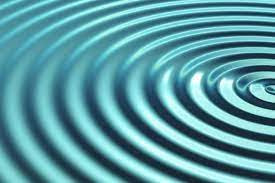
\includegraphics[scale=0.9]{Imagenes/Ondas_01.jpg}
\end{figure}
\end{frame}
\begin{frame}
\frametitle{Las ondas en la naturaleza}
\begin{figure}
    \centering
    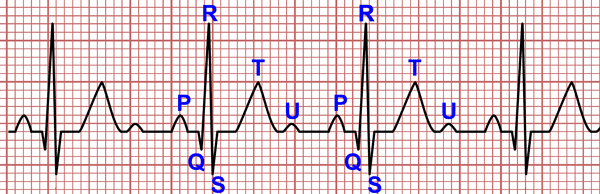
\includegraphics[scale=0.5]{Imagenes/Ondas_02.png}
\end{figure}
\end{frame}
\begin{frame}
\frametitle{Las ondas en la naturaleza}
\begin{figure}
    \centering
    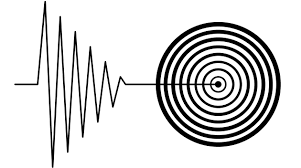
\includegraphics[scale=0.6]{Imagenes/Ondas_03.png}
\end{figure}
\end{frame}

\section{El sonido}
\frame[allowframebreaks]{\tableofcontents[currentsection, hideothersubsections]}
\subsection{El sonido es una onda}

\begin{frame}
\frametitle{¿Cómo explicamos el sonido?}
De manera inicial debemos de considerar que la \textocolor{cobalt}{definición física} del sonido es un concepto, \pause y otro distinto es \textocolor{cadmiumgreen}{la sensación fisiológica} del mismo.
\end{frame}
\begin{frame}
\frametitle{¿Cómo explicamos el sonido?}
Es un \textocolor{blue-violet}{alteración mecánica} que provoca un movimiento ondulatorio a través de \textocolor{red}{medios elásticos} (sólidos, líquidos o gaseosos) en todas las direcciones, \pause en forma de \textocolor{burgundy}{ondas longitudinales} de presión sonora.
\end{frame}
\begin{frame}
\frametitle{El sonido}
Este fenómeno físico tiene su origen en las \textocolor{ao}{vibraciones mecánicas} de la materia, \pause generalmente un sólido que transmite la vibración a las partículas contiguas de aire, u otro medio de propagación, en contacto con el mismo, pero sin arrastrarlas.
\end{frame}
\begin{frame}
\frametitle{El sonido}
Produciendo de forma alternativa \textocolor{awesome}{depresiones} y \textocolor{bondiblue}{sobrepresiones} que se van transmitiendo a las capas de aire adyacentes.
\end{frame}
\begin{frame}
\frametitle{Una onda}
\begin{figure}
\centering
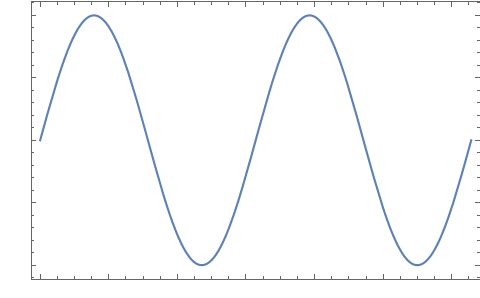
\includegraphics[scale=0.7]{Imagenes/Plot_Onda_01.png}
\end{figure}
\end{frame}
\begin{frame}
\frametitle{El sonido}
Dando lugar a una onda de presión que se propaga con movimiento ondulatorio en todas las direcciones y alejándose del foco. 
\end{frame}
\begin{frame}
\frametitle{Una onda}
\begin{figure}
\centering
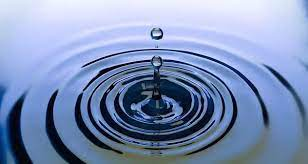
\includegraphics[scale=0.7]{Imagenes/Ondas_04.png}
\end{figure}
\end{frame}
\begin{frame}
\frametitle{Energía en el movimiento}
Cuando el sonido se transmite, hay un \textocolor{coquelicot}{transporte de energía} sin transporte de materia.
\end{frame}

\subsection{Sonido como sensación}

\begin{frame}
\frametitle{El oído y el sonido}
El oído \textocolor{bulgarianrose}{transforma las presiones acústicas} en sensación auditiva.
\end{frame}
\begin{frame}
\frametitle{Sensación auditiva}
Que es aquella engendrada en nuestro oído por una onda acústica y por la tanto siempre con un sentido subjetivo ya que depende del receptor de ésta.
\end{frame}
\begin{frame}
\frametitle{Sensación auditiva}
\begin{figure}
\centering
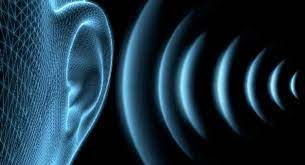
\includegraphics[scale=0.7]{Imagenes/Ondas_05.jpg}
\end{figure}
\end{frame}
\begin{frame}
\frametitle{Sensación auditiva}
Las variaciones de presión generadas por las ondas sonoras provocan la \textocolor{byzantium}{vibración del tímpano}, situado en el oído.
\end{frame}
\begin{frame}
\frametitle{Sensación auditiva}
Transmitiéndose a una cadena de huesecillos, \pause lo que hace que por medio una serie de mecanismos la sensación sonora llegue al cerebro mediante el nervio auditivo.
\end{frame}
% El sonido en sí es de cierta forma una onda.; En cualquier disturbio vibratorio que, propagado a través de un medio elástico, causa una alteración en la presión del medio capaz de producir una sensación auditiva en una persona con audición normal, o de poder ser detectada por un instrumento de captación dentro del rango de frecuencias e intensidades de percepción del oído. Origina en dicho medio una serie de compresiones y enrarecimientos, desplazándose a través de esta a una velocidad que depende de la naturaleza del mismo medio. El sonido se propaga a través de medios gaseosos (Por ejemplo el aire), pero también lo hace en medios líquidos y gaseosos.
% \end{frame}
\section{Una onda}
\frame[allowframebreaks]{\tableofcontents[currentsection, hideothersubsections]}
\subsection{Caracterización de una onda}

\begin{frame}
\frametitle{Propiedades de una onda}
Toda onda mecánica o sonora cuenta con las siguientes propiedades:
\end{frame}
\begin{frame}
\frametitle{Propiedades de una onda}
\setbeamercolor{item projected}{bg=burgundy,fg=white}
\setbeamertemplate{enumerate items}{%
\usebeamercolor[bg]{item projected}%
\raisebox{1.5pt}{\colorbox{bg}{\color{fg}\footnotesize\insertenumlabel}}%
}
\begin{enumerate}[<+->]
\item \textocolor{brown(web)}{Elongación} (y): es la distancia entre la posición de la onda y su posición de equilibrio.
\seti
\end{enumerate}
\end{frame}
\begin{frame}
\frametitle{Elongación de una onda}
\begin{figure}
    \centering
    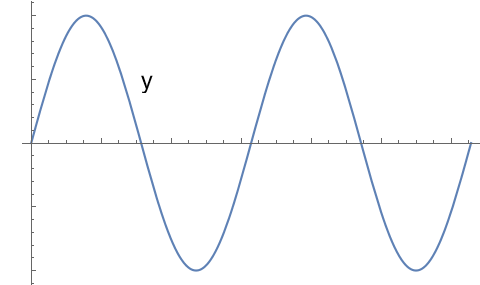
\includegraphics[scale=0.8]{Imagenes/Plot_Onda_02.png}
\end{figure}
\end{frame}
\begin{frame}
\frametitle{Propiedades de una onda}
\setbeamercolor{item projected}{bg=burgundy,fg=white}
\setbeamertemplate{enumerate items}{%
\usebeamercolor[bg]{item projected}%
\raisebox{1.5pt}{\colorbox{bg}{\color{fg}\footnotesize\insertenumlabel}}%
}
\begin{enumerate}[<+->]
\conti
\item \textocolor{cardinal}{Amplitud (A)}: es la distancia entre la elongación máxima y su posición de equilibrio.
\seti
\end{enumerate}
\end{frame}
\begin{frame}
\frametitle{Amplitud de una onda}
\begin{figure}
    \centering
    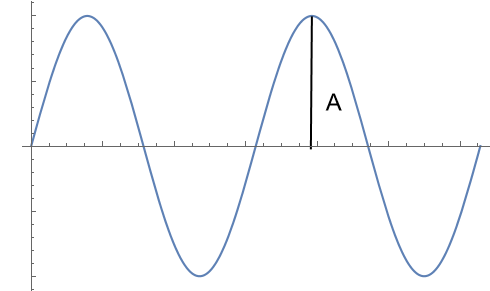
\includegraphics[scale=0.8]{Imagenes/Plot_Onda_03.png}
\end{figure}
\end{frame}
\begin{frame}
\frametitle{Propiedades de una onda}
\setbeamercolor{item projected}{bg=burgundy,fg=white}
\setbeamertemplate{enumerate items}{%
\usebeamercolor[bg]{item projected}%
\raisebox{1.5pt}{\colorbox{bg}{\color{fg}\footnotesize\insertenumlabel}}%
}
\begin{enumerate}[<+->]
\conti
\item \textocolor{carrotorange}{Cresta}: cada uno de los puntos más altos de la onda.
\seti
\end{enumerate}
\end{frame}
\begin{frame}
\frametitle{Cresta de una onda}
\begin{figure}
    \centering
    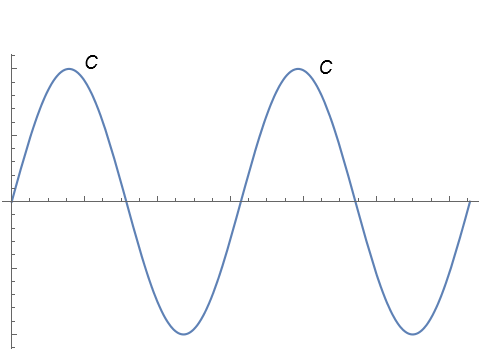
\includegraphics[scale=0.8]{Imagenes/Plot_Onda_04.png}
\end{figure}
\end{frame}
\begin{frame}
\frametitle{Propiedades de una onda}
\setbeamercolor{item projected}{bg=burgundy,fg=white}
\setbeamertemplate{enumerate items}{%
\usebeamercolor[bg]{item projected}%
\raisebox{1.5pt}{\colorbox{bg}{\color{fg}\footnotesize\insertenumlabel}}%
}
\begin{enumerate}[<+->]
\conti
\item \textocolor{darkcyan}{Valle}: cada uno de los puntos más bajos de la onda.
\seti
\end{enumerate}
\end{frame}
\begin{frame}
\frametitle{Valle de una onda}
\begin{figure}
    \centering
    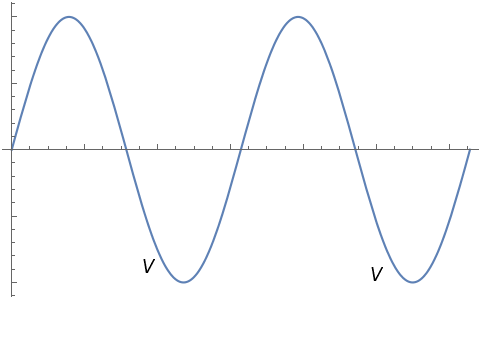
\includegraphics[scale=0.8]{Imagenes/Plot_Onda_05.png}
\end{figure}
\end{frame}
\begin{frame}
\frametitle{Propiedades de una onda}
\setbeamercolor{item projected}{bg=burgundy,fg=white}
\setbeamertemplate{enumerate items}{%
\usebeamercolor[bg]{item projected}%
\raisebox{1.5pt}{\colorbox{bg}{\color{fg}\footnotesize\insertenumlabel}}%
}
\begin{enumerate}[<+->]
\conti
\item \textocolor{cornellred}{Ciclo u oscilación}: es el recorrido de la onda desde un punto hasta el siguiente punto equivalente.
\seti
\end{enumerate}
\end{frame}
\begin{frame}
\frametitle{Ciclo u oscilación}
\begin{figure}
    \centering
    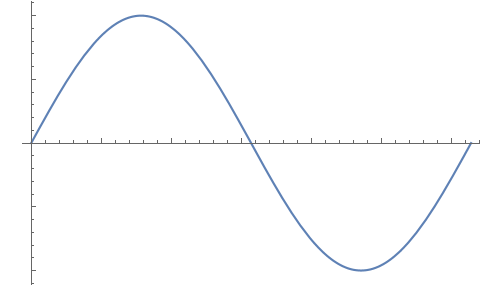
\includegraphics[scale=0.8]{Imagenes/Plot_Onda_06.png}
\end{figure}
\end{frame}
\begin{frame}
\frametitle{Ciclo u oscilación}
\begin{figure}
    \centering
    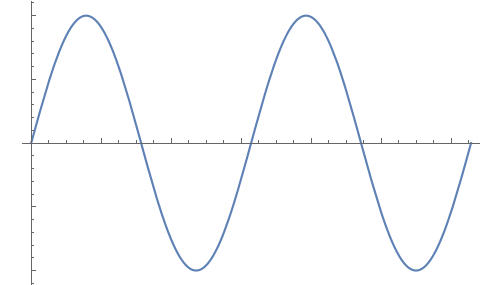
\includegraphics[scale=0.8]{Imagenes/Plot_Onda_06b.png}
\end{figure}
\end{frame}
\begin{frame}
\frametitle{Ciclo u oscilación}
\begin{figure}
    \centering
    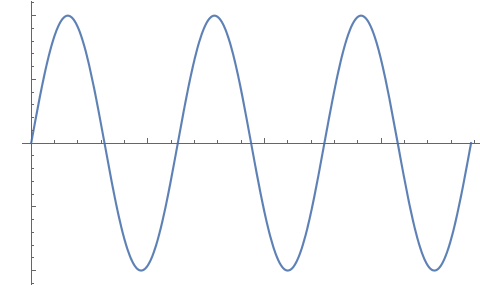
\includegraphics[scale=0.8]{Imagenes/Plot_Onda_06c.png}
\end{figure}
\end{frame}
\begin{frame}
\frametitle{Propiedades de una onda}
\setbeamercolor{item projected}{bg=burgundy,fg=white}
\setbeamertemplate{enumerate items}{%
\usebeamercolor[bg]{item projected}%
\raisebox{1.5pt}{\colorbox{bg}{\color{fg}\footnotesize\insertenumlabel}}%
}
\begin{enumerate}[<+->]
\conti
\item \textocolor{cinnabar}{Longitud de onda ($\lambda$)}: es la distancia que separa dos puntos equivalentes consecutivos de la onda.
\seti
\end{enumerate}
\end{frame}
\begin{frame}
\frametitle{Longitud de onda}
\begin{figure}
    \centering
    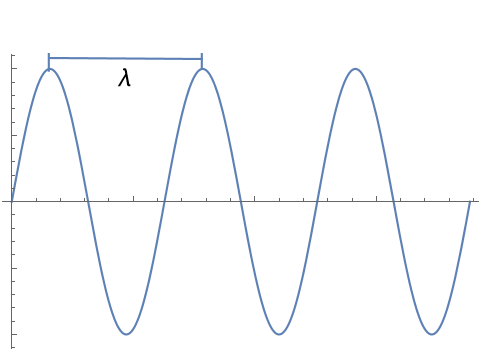
\includegraphics[scale=0.8]{Imagenes/Plot_Onda_07.png}
\end{figure}
\end{frame}
\begin{frame}
\frametitle{Propiedades de una onda}
\setbeamercolor{item projected}{bg=burgundy,fg=white}
\setbeamertemplate{enumerate items}{%
\usebeamercolor[bg]{item projected}%
\raisebox{1.5pt}{\colorbox{bg}{\color{fg}\footnotesize\insertenumlabel}}%
}
\begin{enumerate}[<+->]
\conti
\item \textocolor{cerulean}{Periodo (T)}: es el tiempo que se necesita para hacer una oscilación completa.
\seti
\end{enumerate}
\end{frame}
\begin{frame}
\frametitle{Propiedades de una onda}
\setbeamercolor{item projected}{bg=burgundy,fg=white}
\setbeamertemplate{enumerate items}{%
\usebeamercolor[bg]{item projected}%
\raisebox{1.5pt}{\colorbox{bg}{\color{fg}\footnotesize\insertenumlabel}}%
}
\begin{enumerate}[<+->]
\conti
\item \textocolor{darkorchid}{Frecuencia (f)}: es el número de oscilaciones o vibraciones que realiza la onda por unidad de tiempo.
\\
\bigskip
El período y la frecuencia se relacionan mediante la expresión:
\pause
\begin{align*}
f = \dfrac{1}{T}
\end{align*}
\seti
\end{enumerate}
\end{frame}
\begin{frame}
\frametitle{Propiedades de una onda}
\setbeamercolor{item projected}{bg=burgundy,fg=white}
\setbeamertemplate{enumerate items}{%
\usebeamercolor[bg]{item projected}%
\raisebox{1.5pt}{\colorbox{bg}{\color{fg}\footnotesize\insertenumlabel}}%
}
\begin{enumerate}[<+->]
\conti
\item \textocolor{darkred}{Frecuencia angular ($\omega$)}: es la velocidad a la que la onda realiza las oscilaciones.
\pause
\begin{eqnarray*}
\begin{aligned}
\omega = \dfrac{2 \cdot \pi}{T} = \pause 2 \cdot \pi \cdot f
\end{aligned}
\end{eqnarray*}
\seti
\end{enumerate}
\end{frame}
\begin{frame}
\frametitle{Propiedades de una onda}
\setbeamercolor{item projected}{bg=burgundy,fg=white}
\setbeamertemplate{enumerate items}{%
\usebeamercolor[bg]{item projected}%
\raisebox{1.5pt}{\colorbox{bg}{\color{fg}\footnotesize\insertenumlabel}}%
}
\begin{enumerate}[<+->]
\conti
\item \textocolor{darkviolet}{Velocidad de propagación (v)}: es la velocidad a la que se propaga la onda.
\pause
\begin{eqnarray*}
\begin{aligned}
v = \dfrac{\lambda}{T} = \pause \lambda \cdot f
\end{aligned}
\end{eqnarray*}
\end{enumerate}
\end{frame}

\section{Expresión para una onda}
\frame[allowframebreaks]{\tableofcontents[currentsection, hideothersubsections]}
\subsection{Fórmula matemática}

\begin{frame}
\frametitle{Expresión necesaria}
Toda onda requiere de una expresión general que recupera las propiedades mencionadas previamente.
\end{frame}
\begin{frame}
\frametitle{Expresión matemática}
La función matemática que nos permite describir el movimiento de una onda siempre es de la siguiente forma:
\pause
\begin{align*}
y = f (x \pm v \cdot t)
\end{align*}
\end{frame}
\begin{frame}
\frametitle{Expresión matemática}
\begin{align*}
y = f (x \pm v \cdot t)
\end{align*}
Donde:
\setbeamercolor{item projected}{bg=debianred,fg=white}
\setbeamertemplate{enumerate items}{%
\usebeamercolor[bg]{item projected}%
\raisebox{1.5pt}{\colorbox{bg}{\color{fg}\footnotesize\insertenumlabel}}%
}
\begin{enumerate}[<+->]
\item $y$ es la elongación de la onda.
\item $x$ es la distancia desde el punto estudiado hasta el origen de la onda.
\seti
\end{enumerate}
\end{frame}
\begin{frame}
\frametitle{Expresión matemática}
\begin{align*}
y = f (x \pm v \cdot t)
\end{align*}
\setbeamercolor{item projected}{bg=debianred,fg=white}
\setbeamertemplate{enumerate items}{%
\usebeamercolor[bg]{item projected}%
\raisebox{1.5pt}{\colorbox{bg}{\color{fg}\footnotesize\insertenumlabel}}%
}
\begin{enumerate}[<+->]
\conti
\item $v$ es la velocidad de propagación de la onda.
\item $t$ es el instante de tiempo.
\seti
\end{enumerate}
\end{frame}
\begin{frame}
\frametitle{Expresión matemática}
\begin{align*}
y = f (x \pm v \cdot t)
\end{align*}
\setbeamercolor{item projected}{bg=debianred,fg=white}
\setbeamertemplate{enumerate items}{%
\usebeamercolor[bg]{item projected}%
\raisebox{1.5pt}{\colorbox{bg}{\color{fg}\footnotesize\insertenumlabel}}%
}
\begin{enumerate}[<+->]
\conti
\item El signo delante de la velocidad de propagación indica si la onda mecánica se desplaza hacia la derecha (signo negativo) o hacia la izquierda (signo positivo).
\end{enumerate}
\end{frame}

\subsection{Ejercicios}

\begin{frame}
\frametitle{Resolviendo algunos ejercicios}
Con la finalidad de repasar los conceptos y a la vez, plantear una estrategia para resolver ejercicios, que se recomienda ampliamente para que se ocupe en cada ejercicio.
\end{frame}
\begin{frame}
\frametitle{Procedimiento para resolver un ejercicio}
Se presenta la siguiente estrategia de solución:
\pause
\setbeamercolor{item projected}{bg=cardinal,fg=white}
\setbeamertemplate{enumerate items}{%
\usebeamercolor[bg]{item projected}%
\raisebox{1.5pt}{\colorbox{bg}{\color{fg}\footnotesize\insertenumlabel}}%
}
\begin{enumerate}[<+->]
\item Datos.
\item Expresión(es)
\item Sustitución.
\item Resultado (con unidades)
\end{enumerate}
\end{frame}    
\begin{frame}
\frametitle{Enunciado del Ejercicio 1}
Un péndulo de un metro de longitud oscila con un período de \SI{0.31944}{\second}
\\
\bigskip
\pause
\setbeamercolor{item projected}{bg=bananayellow,fg=ao}
\setbeamertemplate{enumerate items}{%
\usebeamercolor[bg]{item projected}%
\raisebox{1.5pt}{\colorbox{bg}{\color{fg}\footnotesize\insertenumlabel}}%
}
\begin{enumerate}[<+->]
\item ¿Cuál es su frecuencia?
\item ¿Cuántas oscilaciones dará en medio minuto?
\end{enumerate}
\end{frame}
\begin{frame}
\frametitle{Resolviendo el ejercicio 1}
\textocolor{red}{Datos:} \pause Período \, $T = \SI{0.31944}{\second}$
\\
\bigskip
\pause
\textocolor{red}{Expresión(es):}
\pause
\begin{eqnarray*}
\begin{aligned}
f &= \dfrac{1}{T} \\[0.5em] \pause
f &= \dfrac{\text{oscilaciones}}{\text{tiempo}} \pause \hspace{0.5cm} \Rightarrow \hspace{0.5cm} \text{oscilaciones} = f \cdot \text{tiempo}
\end{aligned}
\end{eqnarray*}
\end{frame}
\begin{frame}
\frametitle{Resolviendo el ejercicio 1}
\textocolor{red}{Sustitución:}
\pause
\begin{eqnarray*}
\begin{aligned}
f &= \dfrac{1}{T} = \pause \dfrac{1}{\SI{0.31944}{\second}} = \pause \SI{3.1304}{\hertz} \\[0.5em] \pause
\text{oscilaciones} &= f \cdot \text{tiempo} = \\[0.5em] \pause
&= (\SI{3.1304}{\hertz})(\SI{30}{\second}) = \\[0.5em] \pause 
&= 93.91 \, \text{oscilaciones}
\end{aligned}
\end{eqnarray*}
\end{frame}
\begin{frame}
\frametitle{Enunciado del ejercicio 2}
La frecuencia cardiaca de una persona que está desarrollando una actividad física es de 120 latidos por minuto:
\setbeamercolor{item projected}{bg=byzantium,fg=white}
\setbeamertemplate{enumerate items}{%
\usebeamercolor[bg]{item projected}%
\raisebox{1.5pt}{\colorbox{bg}{\color{fg}\footnotesize\insertenumlabel}}%
}
\begin{enumerate}[<+->]
\item ¿Cúal es su período de oscilación?
\item Si la actividad física duró \SI{35}{\minute}, ¿cuántos latidos dio el corazón?
\end{enumerate}
\end{frame}
\begin{frame}
\frametitle{Resolviendo el ejercicio 2}
\textocolor{red}{Datos}:
\pause
\begin{eqnarray*}
\begin{aligned}
120 \, \text{lpm} \pause \hspace{0.3cm} &\Rightarrow \hspace{0.3cm} \dfrac{120 \, \text{lpm}}{\SI{60}{\second}} \pause \hspace{0.3cm} \Rightarrow \hspace{0.3cm} f = \SI{2}{\hertz} \\[0.5em] \pause
t &= \SI{35}{\minute} = \pause \SI{2100}{\second}
\end{aligned}
\end{eqnarray*}
\end{frame}
\begin{frame}
\frametitle{Resolviendo el ejercicio 2}
\textocolor{red}{Expresiones}:
\begin{eqnarray*}
\begin{aligned}
f &= \dfrac{1}{T} = \pause \hspace{0.5cm} T = \dfrac{1}{f} \\[0.5em] \pause
\text{oscilaciones} &= f \cdot t 
\end{aligned}
\end{eqnarray*}
\end{frame}
\begin{frame}
\frametitle{Resolviendo el ejercicio 2}
\textocolor{red}{Sustitución}:
\begin{eqnarray*}
\begin{aligned}
T &= \dfrac{1}{\SI{2}{\hertz}} = \pause \SI{0.5}{\second} \\[0.5em] \pause
\text{oscilaciones} &= (\SI{2}{\hertz})(\SI{2100}{\second}) = \\[0.5em] \pause
&= \num{4.2d3} \, \text{oscilaciones}
\end{aligned}
\end{eqnarray*}
\end{frame}
\begin{frame}
\frametitle{Enunciado del ejercicio 3}
En un estanque de agua se produce una onda cuya longitud de onda es $\lambda = \SI{17}{\milli\meter}$ y un período de $T = \SI{0.8}{\second}$
\pause
\setbeamercolor{item projected}{bg=aquamarine,fg=black}
\setbeamertemplate{enumerate items}{%
\usebeamercolor[bg]{item projected}%
\raisebox{1.5pt}{\colorbox{bg}{\color{fg}\footnotesize\insertenumlabel}}%
}
\begin{enumerate}[<+->]
\item ¿Cúal será la velocidad de la onda?
\item ¿Qué tiempo le tomará recorrer \SI{2}{\meter}?
\end{enumerate}
\end{frame}
\begin{frame}
\frametitle{Resolviendo el ejercicio 3}
\textocolor{red}{Datos}:
\pause
\begin{eqnarray*}
\begin{aligned}
\lambda &= \SI{17}{\milli\meter} = \pause \SI{17d-3}{\meter}\\[0.5em] \pause
T &= \SI{0.8}{\second} \\[0.5em] \pause
d &= \SI{2}{\meter}
\end{aligned}
\end{eqnarray*}
\end{frame}
\begin{frame}
\frametitle{Resolviendo el ejercicio 3}
\textocolor{red}{Expresiones}:
\begin{eqnarray*}
\begin{aligned}
f &= \dfrac{1}{T} \\[0.5em] \pause
v &= \lambda \cdot f \\[0.5em] \pause
v &= \dfrac{d}{t} \hspace{0.5cm} \Rightarrow \hspace{0.5cm} t = \dfrac{d}{v}
\end{aligned}
\end{eqnarray*}
\end{frame}
\begin{frame}
\frametitle{Resolviendo el ejercicio 3}
\textocolor{red}{Sustitución}:
\begin{eqnarray*}
\begin{aligned}
f &= \dfrac{1}{T} = \dfrac{1}{\SI{0.8}{\second}} = \pause \SI{1.25}{\hertz} \\[0.5em] \pause
v &= \lambda \cdot f = \pause (\SI{17d-3}{\meter})(\SI{1.25}{\hertz}) = \\[0.5em] \pause
&= \SI[per-mode=fraction]{0.02125}{\meter\per\second} = \pause \SI[per-mode=fraction]{2.125d-2}{\meter\per\second} \\[0.5em] \pause
t &= \dfrac{d}{v} = \pause \dfrac{\SI{2}{\meter}}{\SI[per-mode=fraction]{2.125d-2}{\meter\per\second}} = \pause \SI{94.117}{\second}
\end{aligned}
\end{eqnarray*}
\end{frame}
\begin{frame}
\frametitle{Enunciado del ejercicio 4}
En un tanque de agua, la orilla del mismo se encuentra a una distancia de \SI{80}{\centi\meter} del punto donde una piedra cayó, \pause se registra que el tiempo entre la caída de la piedra y la llegada de la onda a la orilla siendo de \SI{12}{\second}.
\end{frame}
\begin{frame}
\frametitle{Enunciado del ejercicio 4}
Si la onda tiene una longitud de onda es de \SI{14}{\milli\meter},
\\
\bigskip
\pause
\setbeamercolor{item projected}{bg=cadmiumgreen,fg=white}
\setbeamertemplate{enumerate items}{%
\usebeamercolor[bg]{item projected}%
\raisebox{1.5pt}{\colorbox{bg}{\color{fg}\footnotesize\insertenumlabel}}%
}
\begin{enumerate}[<+->]
\item ¿Qué velocidad tiene la onda?
\item ¿Cuál es la frecuencia de oscilación?
\end{enumerate}
\end{frame}
\begin{frame}
\frametitle{Resolviendo el ejercicio 4}
\textocolor{red}{Datos}:
\pause
\begin{eqnarray*}
\begin{aligned}
d &= \SI{0.8}{\meter} \\[0.5em] \pause
t &= \SI{12}{\second} \\[0.5em] \pause
\lambda &= \SI{14}{\milli\meter}
\end{aligned}
\end{eqnarray*}
\end{frame}
\begin{frame}
\frametitle{Resolviendo el ejercicio 4}
\textocolor{red}{Expresiones}:
\begin{eqnarray*}
\begin{aligned}
v &= \dfrac{d}{t} \\[0.5em] \pause
f &= \dfrac{v}{\lambda}
\end{aligned}
\end{eqnarray*}
\end{frame}
\begin{frame}
\frametitle{Resolviendo el ejercicio 4}
\textocolor{red}{Sustitución}:
\begin{eqnarray*}
\begin{aligned}
v &= \dfrac{d}{t} = \pause \dfrac{\SI{0.8}{\meter}}{\SI{12}{\second}} = \pause \SI[per-mode=fraction]{6.66667d-2}{\meter\per\second} \\[1em] \pause
f &= \dfrac{v}{\lambda} = \pause \dfrac{\SI[per-mode=fraction]{6.66667d-2}{\meter\per\second}}{\SI{14d-3}{\meter}} = \\[0.5em] \pause
&= \SI{4.7619}{\hertz}
\end{aligned}
\end{eqnarray*}
\end{frame}
\begin{frame}
\frametitle{Actividad de evaluación continua}
Hay que resolver $8$ ejercicios como actividad de repaso.
\\
\bigskip
\pause
La fecha de entrega es el domingo 17 de septiembre a las 5 pm, vía Teams.
\end{frame}

\section{Tipos de ondas}
\frame[allowframebreaks]{\tableofcontents[currentsection, hideothersubsections]}
\subsection{Dirección de las ondas}

\begin{frame}
\frametitle{La importancia de la dirección}
De acuerdo con la \textocolor{darkgreen}{dirección} en la que una onda hace vibrar a las partículas del medio material, \pause los movimientos ondulatorios se clasifican en: \textocolor{ginger}{longitudinales} \pause y \textocolor{green(munsell)}{transversales}.
\end{frame}

\subsection{Ondas longitudinales}

\begin{frame}
\frametitle{Definición de ondas longitudinales}
Se presentan cuando las partículas del medio material vibran \textocolor{halayaube}{paralelamente} a la dirección de propagación de la onda.
\end{frame}
\begin{frame}
\frametitle{Onda longitudinal}
\begin{figure}
    \centering
    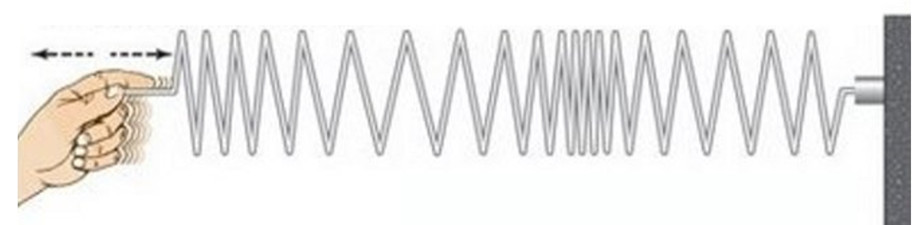
\includegraphics[scale=0.35]{Imagenes/Ondas_07.jpg}
\end{figure}
\end{frame}
\begin{frame}
\frametitle{Propiedades de una onda longitudinal}
Ahora revisaremos un par de propiedades importantes de las ondas longitudinales, la \textocolor{cadetblue!80!black}{compresión} \pause y la \textocolor{officegreen}{rarefacción}.
\end{frame}
\begin{frame}
\frametitle{Una onda longitudinal}
\begin{figure}
    \centering
    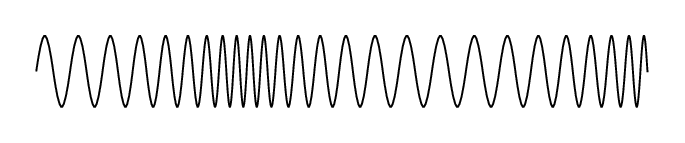
\includegraphics[scale=0.5]{Imagenes/Reflexion_Ondas_05.png}
\end{figure}
\end{frame}
\begin{frame}
\frametitle{Regiones en la onda}
De la figura anterior, reconocemos dos regiones de interés en la onda:
\pause
\setbeamercolor{item projected}{bg=junglegreen,fg=black}
\setbeamertemplate{enumerate items}{%
\usebeamercolor[bg]{item projected}%
\raisebox{1.5pt}{\colorbox{bg}{\color{fg}\footnotesize\insertenumlabel}}%
}
\begin{enumerate}[<+->]
\item Compresión.
\item Rarefaccción (expansión).
\end{enumerate}
\end{frame}
\begin{frame}
\frametitle{Reflexión de una onda}
\begin{figure}
    \centering
    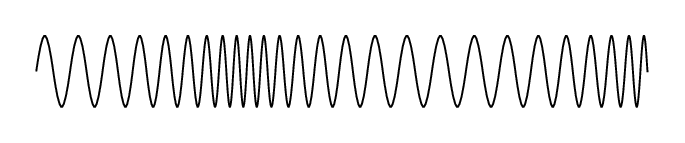
\includegraphics[scale=0.7]{Imagenes/Reflexion_Ondas_05.png}
\end{figure}
\begin{tikzpicture}[overlay]
    \draw [line width=0.1cm, color=lavenderindigo] (1.5, 4.5) -- (4.8, 4.5) node [above, midway] {Rarefacción};
    \draw [line width=0.1cm, color=lava] (5.2, 4.5) -- (6.8, 4.5) node [above, midway] {Compresión};
\end{tikzpicture}
\end{frame}
    
% Tal es el caso de las ondas producidas en un resorte,
% como el de la figura 10.1, el cual se comporta como un oscilador
% armónico cuando se tira del cuerpo suspendido en
% su parte inferior y comienza a oscilar de abajo hacia arriba,
% produciendo ondas longitudinales.
% \end{frame}

\subsection{Ondas transversales}

\begin{frame}
\frametitle{Definición de ondas transversales}
Se presentan cuando las partículas del medio material vibran \textocolor{navyblue}{perpendicularmente} a la dirección de propagación de la onda.
\end{frame}
\begin{frame}
\frametitle{Onda transversal}
\begin{figure}
    \centering
    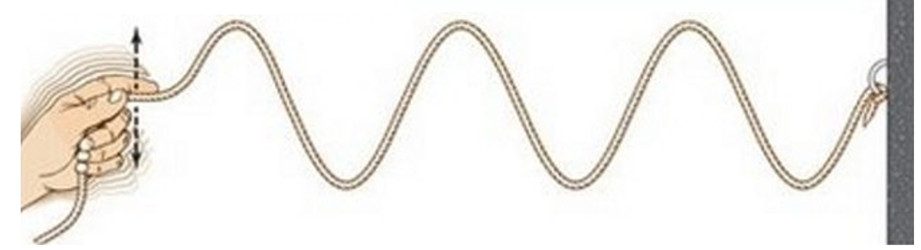
\includegraphics[scale=0.35]{Imagenes/Ondas_08.jpg}
\end{figure}
\end{frame}
\begin{frame}
\frametitle{Ejemplo de ondas transversales}
Éstas se producen, por ejemplo, cuando se arroja una piedra en un estanque; \pause al entrar en el agua, expulsa el líquido en todas direcciones; \pause por tanto, unas moléculas empujan a otras, formándose prominencias y depresiones circulares alrededor de la piedra.
\end{frame}
\begin{frame}
\frametitle{Ondas transversales}
\begin{figure}
    \centering
    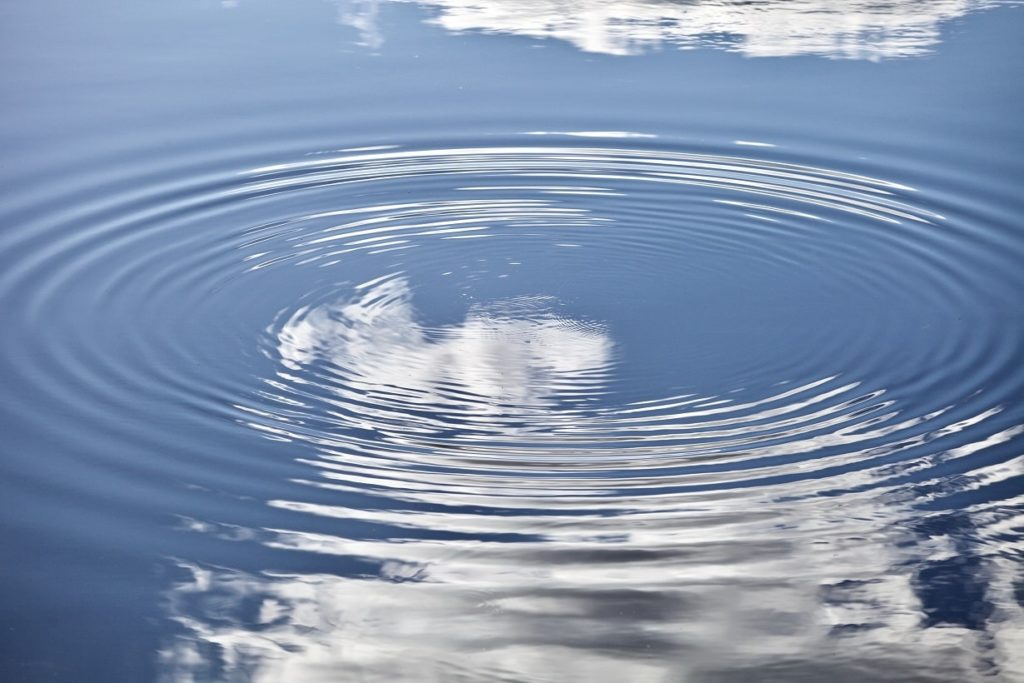
\includegraphics[scale=0.25]{Imagenes/Ondas_06.jpg}
\end{figure}
\end{frame}
\begin{frame}
\frametitle{Ejemplo de ondas transversales}
Como las moléculas de agua vibran (oscilan), hacia arriba y hacia abajo, en forma perpendicular
a la dirección en la que se propaga la onda, \pause ésta recibe el nombre de transversal.
\end{frame}

\subsection{Energía y ondas}

\begin{frame}
\frametitle{Relación entre energía y ondas}
En las ondas mecánicas la que se desplaza o avanza es la \textocolor{red}{energía} de la onda y no las partículas del medio, pues éstas únicamente vibran u oscilan transmitiendo la energía, pero conservan sus posiciones alrededor de puntos más o menos fijos.
\end{frame}
\begin{frame}
\frametitle{Relación entre energía y ondas}    
En general, las ondas mecánicas transmiten la energía por medio de la materia, debido a las perturbaciones ocasionadas en ella, pero sin que implique un desplazamiento total de la materia.
\end{frame}


\section{Ondas en movimiento}
\frame[allowframebreaks]{\tableofcontents[currentsection, hideothersubsections]}
\subsection{Reflexión}

\begin{frame}
\frametitle{La reflexión de ondas}
La \textocolor{carmine}{reflexión} de las ondas se presenta cuando éstas encuentran un obstáculo que les impide propagarse, \pause chocan y cambian de sentido sin modificar sus demás características.
\end{frame}
\begin{frame}
\frametitle{La reflexión de ondas}
En las siguientes figuras vemos cómo se refleja una onda lineal en donde uno de los \textocolor{coquelicot}{extremos está fijo}.
\end{frame}
\begin{frame}
\frametitle{Reflexión de una onda}
\begin{figure}
    \centering
    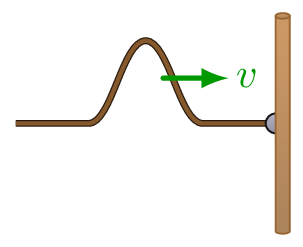
\includegraphics[scale=0.7]{Imagenes/Reflexion_Ondas_01.png}
\end{figure}
\end{frame}
\begin{frame}
\frametitle{Reflexión de una onda}
\begin{figure}
    \centering
    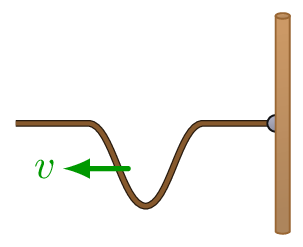
\includegraphics[scale=0.7]{Imagenes/Reflexion_Ondas_02.png}
\end{figure}
\end{frame}
\begin{frame}
\frametitle{Reflexión con un extremo móvil}
En las siguientes figuras veremos cómo se presenta la reflexión de una onda, donde uno de los \textocolor{darkmagenta}{extremos no está fijo}.
\end{frame}
\begin{frame}
\frametitle{Reflexión de una onda}
\begin{figure}
    \centering
    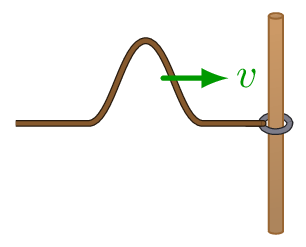
\includegraphics[scale=0.7]{Imagenes/Reflexion_Ondas_03.png}
\end{figure}
\end{frame}
\begin{frame}
\frametitle{Reflexión de una onda}
\begin{figure}
    \centering
    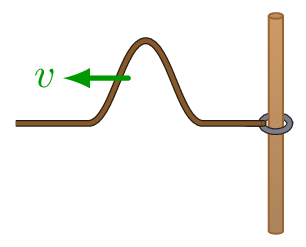
\includegraphics[scale=0.7]{Imagenes/Reflexion_Ondas_04.png}
\end{figure}
\end{frame}
% Una onda producida en un estanque también se refleja al chocar.
%  El ángulo de reflexión de la onda es igual al ángulo
% de choque.
% \end{frame}

\section{Superposición}
\frame[allowframebreaks]{\tableofcontents[currentsection, hideothersubsections]}
\subsection{Tren de ondas}

\begin{frame}
\frametitle{Tren de ondas}
Si a una cuerda tensa y sujeta por uno de sus extremos se le da un impulso moviéndola hacia arriba, se produce una onda que avanza por las partículas de la cuerda.
\end{frame}
\begin{frame}
\frametitle{Tren de ondas}
Éstas ondas se moverán al llegarles el impulso y recobrarán su posición de reposo cuando la onda pase por ellas.
\end{frame}
\begin{frame}
\frametitle{Tren de ondas}
Si la cuerda se sigue moviendo hacia arriba y hacia abajo, producirá un \textocolor{red}{tren de ondas} periódico si el movimiento también es periódico.
\end{frame}
\begin{frame}
\frametitle{Tren de onda}
\begin{figure}
    \centering
    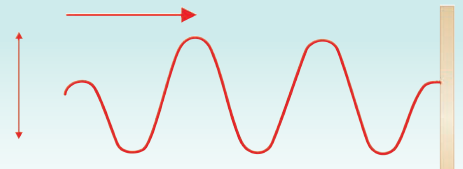
\includegraphics[scale=0.8]{Imagenes/Tren_Onda_01.png}
\end{figure}
\end{frame}
\begin{frame}
\frametitle{Frente de onda}
Al dejar caer una piedra en un estanque, como ya mencionamos, se forman ondas transversales.
\end{frame}
\begin{frame}
\frametitle{Frente de onda}
\begin{figure}
    \centering
    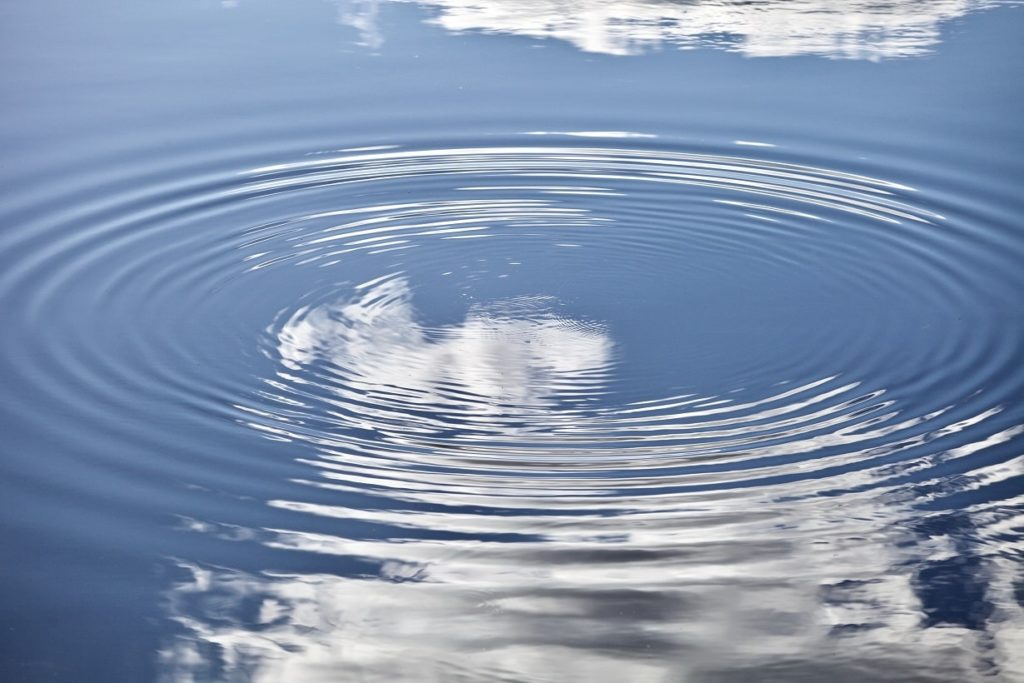
\includegraphics[scale=0.25]{Imagenes/Ondas_06.jpg}
\end{figure}
\end{frame}
\begin{frame}
\frametitle{Frente de onda}
Si los círculos de la imagen anterior representan todos los puntos de una onda que experimentan la misma fase, \pause ya sea una cresta o un valle, \pause al propagarse la onda los círculos se desplazarán generando otros de mayor tamaño. 
\end{frame}
\begin{frame}
\frametitle{Frente de onda}
Cada círculo representa un \textocolor{coquelicot}{frente de onda} formado por todos los puntos de la onda con la misma fase, \pause por eso puede decirse que cada punto de un frente de onda es un nuevo \textocolor{darkblue}{generador de ondas}.
\end{frame}
\begin{frame}
\frametitle{Frente de onda}
A partir del centro emisor de las ondas, es decir, del lugar donde cayó la piedra, los diferentes frentes de una onda \textocolor{americanrose}{avanzan al mismo tiempo} \pause y con una \textocolor{auburn}{magnitud de velocidad constante}.
\end{frame}
\begin{frame}
\frametitle{Rayo/vector de propagación}
Es la \textocolor{burgundy}{línea que señala la dirección} en que avanza cualquiera de los puntos de un frente de onda.
\end{frame}
\begin{frame}
\frametitle{Rayo/vector de propagación}
Cuando el medio en que se propaga la onda es homogéneo, la dirección de los rayos siempre es \textocolor{blue}{perpendicular} o normal al frente de onda.
\end{frame}
\begin{frame}
\frametitle{Rayo/vector de propagación}
\begin{figure}
    \centering
    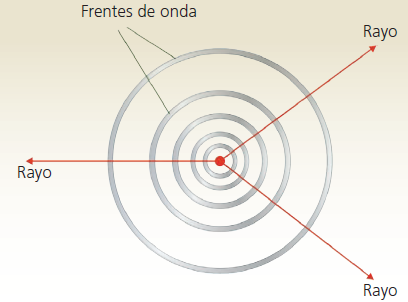
\includegraphics[scale=0.8]{Imagenes/Frente_Onda_01.png}
\end{figure}
\end{frame}

\subsection{Principio de superposición}

\begin{frame}
\frametitle{Propagación de la onda}
Experimentalmente se ha comprobado que al producirse \textocolor{darkscarlet}{dos o más trenes de onda} al mismo tiempo, \pause en medios elásticos que conservan una \textocolor{ferrarired}{proporcionalidad} entre la \textocolor{drab}{deformación} y la \textocolor{dukeblue}{fuerza restauradora}, cada onda se propaga en forma independiente.
\end{frame}
\begin{frame}
\frametitle{Propagación de la onda}
Por tanto, la \textocolor{firebrick}{superposición} es el desplazamiento que experimenta una partícula vibrante, \pause equivalente a la suma vectorial de los desplazamientos que cada onda le produce.
\end{frame}
\begin{frame}
\frametitle{Utilidad del principio de superposición}
Una aplicación útil de este principio se presenta cuando desea estudiarse un movimiento ondulatorio formado por muchos trenes de onda para lo cual se descompone en cada uno de sus trenes constituyentes.
\end{frame}
\begin{frame}
\frametitle{Análisis de tren de ondas}
\begin{figure}
    \centering
    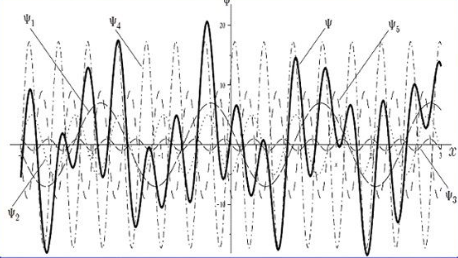
\includegraphics[scale=0.7]{Imagenes/Tren_Onda_02.png}
\end{figure}
\end{frame}


\section{Interferencia de ondas}
\frame[allowframebreaks]{\tableofcontents[currentsection, hideothersubsections]}
\subsection{Definición}

\begin{frame}
\frametitle{Definición de Interferencia}
La \textocolor{carminered}{interferencia} se produce cuando se superponen simultáneamente dos o más trenes de onda; \pause este fenómeno se emplea para comprobar si un movimiento es ondulatorio o no.
\end{frame}

\subsection{Interferencia constructiva}

\begin{frame}
\frametitle{La interferencia constructiva}
La \textocolor{crimsonglory}{interferencia constructiva} se presenta al superponerse dos movimientos ondulatorios de la misma frecuencia y longitud de onda, que llevan el mismo sentido.
\end{frame}
\begin{frame}
\frametitle{La interferencia constructiva}
Las dos ondas superpuestas se representan por medio de líneas punteadas en la siguiente figura:
\end{frame}
\begin{frame}
\frametitle{La interferencia constructiva}
\begin{figure}
    \centering
    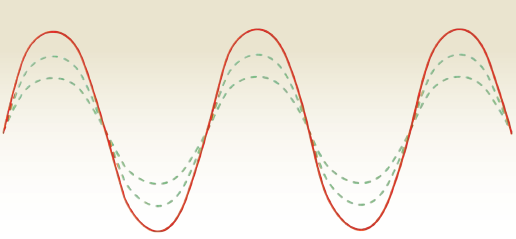
\includegraphics[scale=0.8]{Imagenes/Onda_Constructiva.png}
\end{figure}
\end{frame}

\subsection{Interferencia destructiva}

\begin{frame}
\frametitle{La interferencia destructiva}
La \textocolor{amaranth}{interferencia destructiva} se presenta cuando se superponen dos movimientos ondulatorios con una diferencia de fase.
\end{frame}
\begin{frame}
\frametitle{Caso de interferencia destructiva}
Por ejemplo, al superponerse una cresta y un valle de diferente amplitud con una diferencia de fase igual a
media longitud de onda, \pause la onda resultante tendrá menor amplitud.
\end{frame}
\begin{frame}
\frametitle{Caso de interferencia destructiva}
\begin{figure}
    \centering
    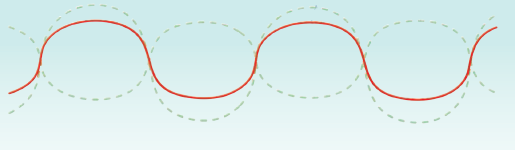
\includegraphics[scale=0.8]{Imagenes/Interferencia_Desctructiva_02.png}
\end{figure}
\end{frame}
\begin{frame}
\frametitle{Otro caso de interferencia destructiva}
Pero si se superponen dos ondas de la misma amplitud con una diferencia de fase equivalente a media longitud de onda, es decir $\ang{180}$, \pause la suma vectorial de sus amplitudes contrarias será igual a cero, \pause  por consiguiente, la onda resultante tendrá una amplitud nula.
\end{frame}
\begin{frame}
\frametitle{Otro caso de interferencia destructiva}
\begin{figure}
    \centering
    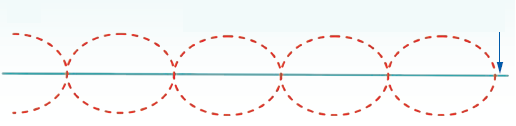
\includegraphics[scale=0.8]{Imagenes/Interferencia_Desctructiva_03.png}
\end{figure}
\end{frame}

\section{Ondas estacionarias}
\frame[allowframebreaks]{\tableofcontents[currentsection, hideothersubsections]}
\subsection{Definición}

\begin{frame}
\frametitle{Las ondas estacionarias}
Las \textocolor{blue(ryb)}{ondas estacionarias} se producen cuando interfieren dos movimientos ondulatorios de la misma \textocolor{brickred}{frecuencia} y \textocolor{byzantium}{amplitud} \pause que se propagan en \textocolor{cadmiumorange}{diferente sentido} a lo largo de una línea \pause con una \textocolor{cobalt}{diferencia de fase} de media longitud de onda.
\end{frame}

\section{Refracción de ondas}
\frame[allowframebreaks]{\tableofcontents[currentsection, hideothersubsections]}
\subsection{Definición de la Refracción}

\begin{frame}
\frametitle{La refracción de ondas}
La \textocolor{atomictangerine}{refracción de ondas} se presenta cuando éstas pasan de un medio a otro de \textcolor{bistre}{distinta densidad}.
\end{frame}
\begin{frame}
\frametitle{La refracción de ondas}
También cuando el medio es el mismo, pero se encuentra en condiciones diferentes, \pause por ejemplo, el agua a distintas profundidades.
\end{frame}
\begin{frame}
\frametitle{La refracción de ondas}
Ello origina que las ondas cambien su \textocolor{cobalt}{magnitud de velocidad} de propagación y su \textocolor{darkcyan}{longitud de onda}, conservando \textocolor{bronze}{constante su frecuencia}.
\end{frame}
\begin{frame}
\frametitle{La refracción de ondas}
Consideremos que un tren de ondas periódico cruza la zona entre dos medios de distinta densidad.
\begin{figure}
    \centering
    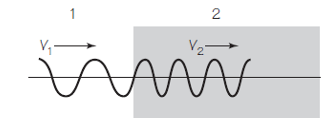
\includegraphics[scale=1]{Imagenes/Refraccion_Ondas_02.png}
\end{figure}
\end{frame}
\begin{frame}
\frametitle{Suposición para la refracción de ondas}    
\begin{figure}
    \centering
    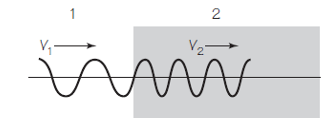
\includegraphics[scale=1]{Imagenes/Refraccion_Ondas_02.png}
\end{figure}
\setbeamercolor{item projected}{bg=black,fg=white}
\setbeamertemplate{enumerate items}{%
\usebeamercolor[bg]{item projected}%
\raisebox{1.5pt}{\colorbox{bg}{\color{fg}\footnotesize\insertenumlabel}}%
}
\begin{enumerate}[<+->]
\item La velocidad de la propagación en el medio 1 es mayor que en el medio 2.
\seti
\end{enumerate}
\end{frame}
\begin{frame}
\frametitle{Suposición para la refracción de ondas}    
\begin{figure}
    \centering
    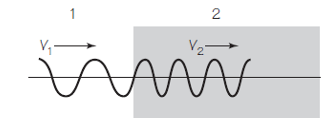
\includegraphics[scale=1]{Imagenes/Refraccion_Ondas_02.png}
\end{figure}
\setbeamercolor{item projected}{bg=black,fg=white}
\setbeamertemplate{enumerate items}{%
\usebeamercolor[bg]{item projected}%
\raisebox{1.5pt}{\colorbox{bg}{\color{fg}\footnotesize\insertenumlabel}}%
}
\begin{enumerate}[<+->]    
\conti
\item Para simplificar suponemos que toda la onda se transmite y nada se refleja.
\end{enumerate}
\end{frame}
\begin{frame}
\frametitle{La refracción de ondas}
El patrón de onda periódico también se comprime.
\begin{figure}
    \centering
    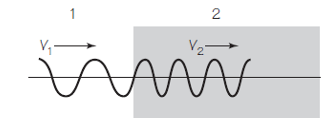
\includegraphics[scale=1]{Imagenes/Refraccion_Ondas_02.png}
\end{figure}
\end{frame}
\begin{frame}
\frametitle{La refracción de ondas}
Por lo tanto, la longitud de onda $\lambda_{2}$ de \textocolor{red}{la onda transmitida es más corta} que la longitud de onda $\lambda_{1}$ de la onda entrante o incidente.
\begin{figure}
    \centering
    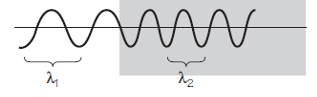
\includegraphics[scale=1]{Imagenes/Refraccion_Ondas_03.png}
\end{figure}
\end{frame}
\begin{frame}
\frametitle{Revisando el caso de la refracción}
Aunque la \textocolor{cordovan}{longitud de onda cambia} cuando la onda pasa a través del límite, \pause la \textocolor{ao}{frecuencia de la onda no puede cambiar}.
\end{frame}
\begin{frame}
\frametitle{Revisando el caso de la refracción}
Si el medio es continuo (una cuerda que no está rota), ambos lados del límite deben subir y bajar juntos.
\end{frame}
\begin{frame}
\frametitle{Revisando el caso de la refracción}
Las frecuencias de las ondas incidentes y transmitidas deben, entonces, \textocolor{darkscarlet}{ser iguales}.
\\
\bigskip
\pause
Podemos simplemente etiquetar ambas como $f$.
\end{frame}
\begin{frame}
\frametitle{Revisando el caso de la refracción}
La relación entre longitud de onda, frecuencia y velocidad para las ondas incidentes y transmitidas se puede escribir por separado como:
\pause
\begin{align*}
\lambda_{1} \, f &= v_{1} \\[0.5em]
\lambda_{2} \, f &= v_{2}
\end{align*}
\end{frame}
\begin{frame}
\frametitle{Revisando el caso de la refracción}    
Dividiendo una ecuación por la otra, eliminado $f$, obtenemos que:
\pause
\begin{align*}
\dfrac{\lambda_1}{\lambda_{2}} = \dfrac{v_{1}}{v_{2}}
\end{align*}
\end{frame}
\begin{frame}
\frametitle{Resultado con la Refracción}
La ecuación anterior nos dice que la razón entre las longitudes de onda en dos medios es igual a la razón entre las velocidades de propagación de las ondas en esos medios.
\end{frame}

\section{Difracción de ondas}
\frame[allowframebreaks]{\tableofcontents[currentsection, hideothersubsections]}
\subsection{Definición de la difracción}

\begin{frame}
\frametitle{¿Qué es la difracción?}
Cuando una onda encuentra un obstáculo en su camino y lo rodea o sigue su contorno \pause se produce \textocolor{ao(english)}{la difracción de ondas}.
\end{frame}
\begin{frame}
\frametitle{Difracción de ondas}
\begin{figure}
    \centering
    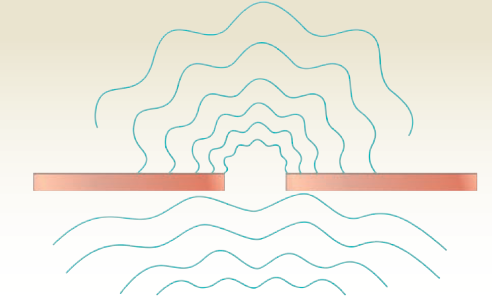
\includegraphics[scale=0.6]{Imagenes/Difraccion_01.PNG}
\end{figure}
\end{frame}
\begin{frame}
\frametitle{La difracción en evidencia}    
Este fenómeno es más notorio a medida que son mayores las longitudes de onda, y si el tamaño de la abertura por la que atravesará la onda es menor.
\end{frame}
\begin{frame}
\frametitle{Grandes aberturas - Poca difracción}
\begin{figure}
    \centering
    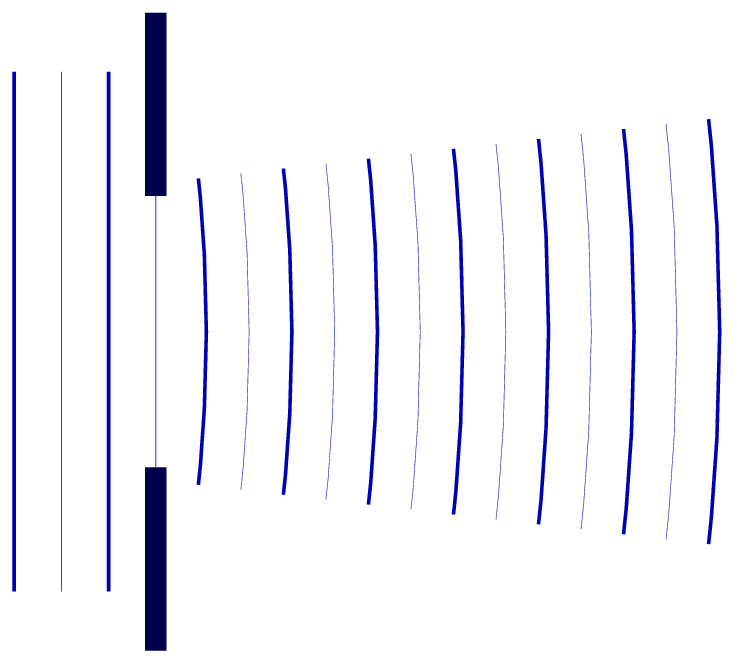
\includegraphics[scale=0.25]{Imagenes/Difraccion_Patrones_01.png}
\end{figure}
\end{frame}
\begin{frame}
\frametitle{No hay abertura - La onda rodea}
\begin{figure}
    \centering
    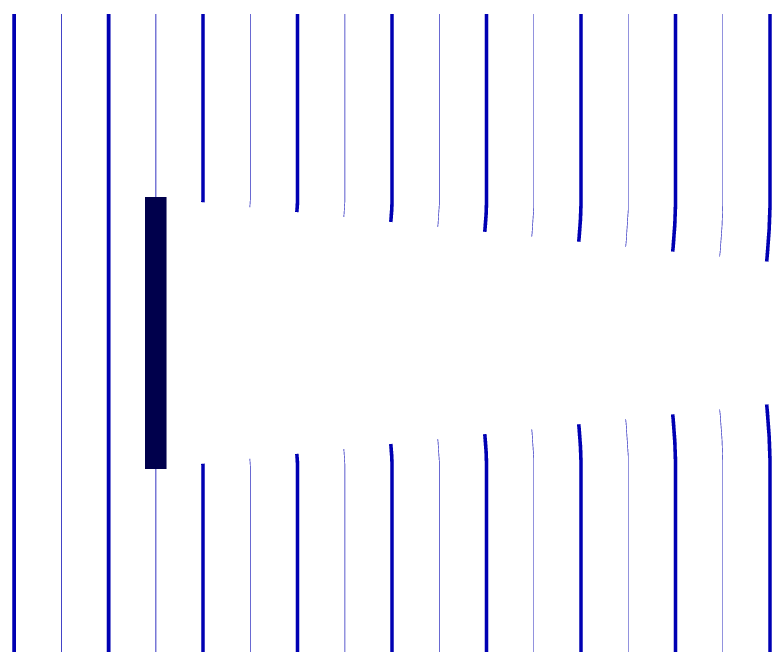
\includegraphics[scale=0.25]{Imagenes/Difraccion_Patrones_02.png}
\end{figure}
\end{frame}
\begin{frame}
\frametitle{Pequeñas aberturas - Mucha difracción}
\begin{figure}
    \centering
    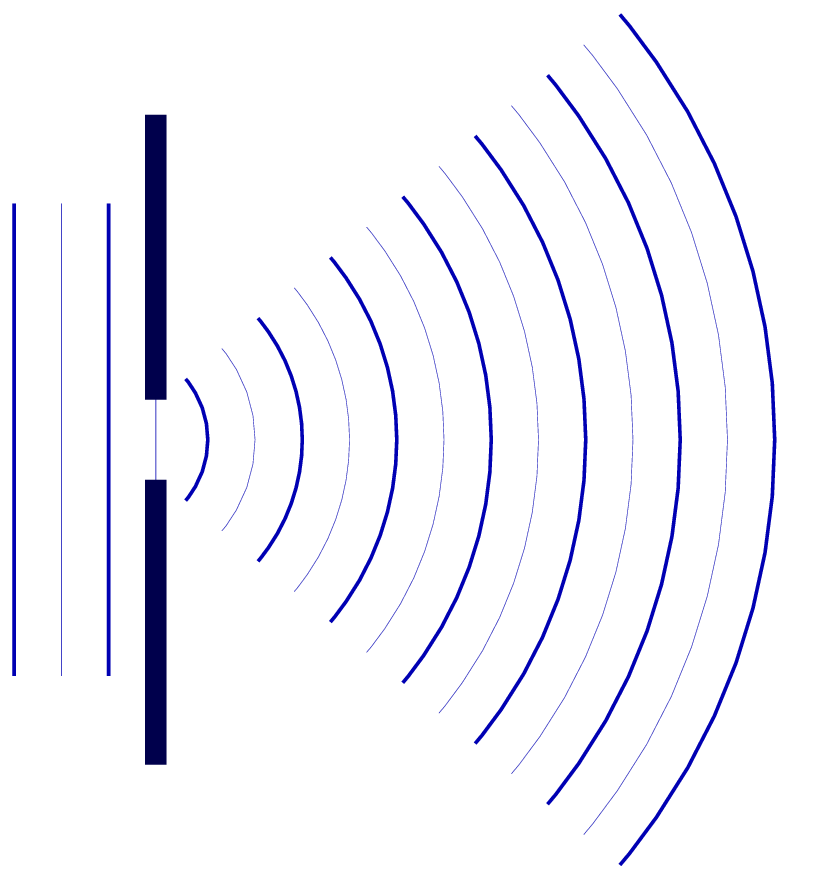
\includegraphics[scale=0.15]{Imagenes/Difraccion_Patrones_03.png}
\end{figure}
\end{frame}
% \begin{frame}
% \frametitle{La difracción en evidencia}
% Longitudes de onda grandes - Mucha difracción
% \begin{figure}
%     \centering
%     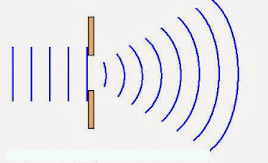
\includegraphics[scale=2.5]{Imagenes/Difraccion_05.jpg}
% \end{figure}
% \end{frame}

\end{document}